% Options for packages loaded elsewhere
% Options for packages loaded elsewhere
\PassOptionsToPackage{unicode}{hyperref}
\PassOptionsToPackage{hyphens}{url}
\PassOptionsToPackage{dvipsnames,svgnames,x11names}{xcolor}
\PassOptionsToPackage{space}{xeCJK}
%
\documentclass[
  chinese-hans,
  letterpaper,
  DIV=11,
  numbers=noendperiod]{scrartcl}
\usepackage{xcolor}
\usepackage{amsmath,amssymb}
\setcounter{secnumdepth}{5}
\usepackage{iftex}
\ifPDFTeX
  \usepackage[T1]{fontenc}
  \usepackage[utf8]{inputenc}
  \usepackage{textcomp} % provide euro and other symbols
\else % if luatex or xetex
  \usepackage{unicode-math} % this also loads fontspec
  \defaultfontfeatures{Scale=MatchLowercase}
  \defaultfontfeatures[\rmfamily]{Ligatures=TeX,Scale=1}
\fi
\usepackage{lmodern}
\ifPDFTeX\else
  % xetex/luatex font selection
  \ifXeTeX
    \usepackage{xeCJK}
    \setCJKmainfont[]{HarmonyOS Sans SC}
  \fi
  \ifLuaTeX
    \usepackage[]{luatexja-fontspec}
    \setmainjfont[]{HarmonyOS Sans SC}
  \fi
\fi
% Use upquote if available, for straight quotes in verbatim environments
\IfFileExists{upquote.sty}{\usepackage{upquote}}{}
\IfFileExists{microtype.sty}{% use microtype if available
  \usepackage[]{microtype}
  \UseMicrotypeSet[protrusion]{basicmath} % disable protrusion for tt fonts
}{}
\makeatletter
\@ifundefined{KOMAClassName}{% if non-KOMA class
  \IfFileExists{parskip.sty}{%
    \usepackage{parskip}
  }{% else
    \setlength{\parindent}{0pt}
    \setlength{\parskip}{6pt plus 2pt minus 1pt}}
}{% if KOMA class
  \KOMAoptions{parskip=half}}
\makeatother
% Make \paragraph and \subparagraph free-standing
\makeatletter
\ifx\paragraph\undefined\else
  \let\oldparagraph\paragraph
  \renewcommand{\paragraph}{
    \@ifstar
      \xxxParagraphStar
      \xxxParagraphNoStar
  }
  \newcommand{\xxxParagraphStar}[1]{\oldparagraph*{#1}\mbox{}}
  \newcommand{\xxxParagraphNoStar}[1]{\oldparagraph{#1}\mbox{}}
\fi
\ifx\subparagraph\undefined\else
  \let\oldsubparagraph\subparagraph
  \renewcommand{\subparagraph}{
    \@ifstar
      \xxxSubParagraphStar
      \xxxSubParagraphNoStar
  }
  \newcommand{\xxxSubParagraphStar}[1]{\oldsubparagraph*{#1}\mbox{}}
  \newcommand{\xxxSubParagraphNoStar}[1]{\oldsubparagraph{#1}\mbox{}}
\fi
\makeatother

\usepackage{color}
\usepackage{fancyvrb}
\newcommand{\VerbBar}{|}
\newcommand{\VERB}{\Verb[commandchars=\\\{\}]}
\DefineVerbatimEnvironment{Highlighting}{Verbatim}{commandchars=\\\{\}}
% Add ',fontsize=\small' for more characters per line
\usepackage{framed}
\definecolor{shadecolor}{RGB}{241,243,245}
\newenvironment{Shaded}{\begin{snugshade}}{\end{snugshade}}
\newcommand{\AlertTok}[1]{\textcolor[rgb]{0.68,0.00,0.00}{#1}}
\newcommand{\AnnotationTok}[1]{\textcolor[rgb]{0.37,0.37,0.37}{#1}}
\newcommand{\AttributeTok}[1]{\textcolor[rgb]{0.40,0.45,0.13}{#1}}
\newcommand{\BaseNTok}[1]{\textcolor[rgb]{0.68,0.00,0.00}{#1}}
\newcommand{\BuiltInTok}[1]{\textcolor[rgb]{0.00,0.23,0.31}{#1}}
\newcommand{\CharTok}[1]{\textcolor[rgb]{0.13,0.47,0.30}{#1}}
\newcommand{\CommentTok}[1]{\textcolor[rgb]{0.37,0.37,0.37}{#1}}
\newcommand{\CommentVarTok}[1]{\textcolor[rgb]{0.37,0.37,0.37}{\textit{#1}}}
\newcommand{\ConstantTok}[1]{\textcolor[rgb]{0.56,0.35,0.01}{#1}}
\newcommand{\ControlFlowTok}[1]{\textcolor[rgb]{0.00,0.23,0.31}{\textbf{#1}}}
\newcommand{\DataTypeTok}[1]{\textcolor[rgb]{0.68,0.00,0.00}{#1}}
\newcommand{\DecValTok}[1]{\textcolor[rgb]{0.68,0.00,0.00}{#1}}
\newcommand{\DocumentationTok}[1]{\textcolor[rgb]{0.37,0.37,0.37}{\textit{#1}}}
\newcommand{\ErrorTok}[1]{\textcolor[rgb]{0.68,0.00,0.00}{#1}}
\newcommand{\ExtensionTok}[1]{\textcolor[rgb]{0.00,0.23,0.31}{#1}}
\newcommand{\FloatTok}[1]{\textcolor[rgb]{0.68,0.00,0.00}{#1}}
\newcommand{\FunctionTok}[1]{\textcolor[rgb]{0.28,0.35,0.67}{#1}}
\newcommand{\ImportTok}[1]{\textcolor[rgb]{0.00,0.46,0.62}{#1}}
\newcommand{\InformationTok}[1]{\textcolor[rgb]{0.37,0.37,0.37}{#1}}
\newcommand{\KeywordTok}[1]{\textcolor[rgb]{0.00,0.23,0.31}{\textbf{#1}}}
\newcommand{\NormalTok}[1]{\textcolor[rgb]{0.00,0.23,0.31}{#1}}
\newcommand{\OperatorTok}[1]{\textcolor[rgb]{0.37,0.37,0.37}{#1}}
\newcommand{\OtherTok}[1]{\textcolor[rgb]{0.00,0.23,0.31}{#1}}
\newcommand{\PreprocessorTok}[1]{\textcolor[rgb]{0.68,0.00,0.00}{#1}}
\newcommand{\RegionMarkerTok}[1]{\textcolor[rgb]{0.00,0.23,0.31}{#1}}
\newcommand{\SpecialCharTok}[1]{\textcolor[rgb]{0.37,0.37,0.37}{#1}}
\newcommand{\SpecialStringTok}[1]{\textcolor[rgb]{0.13,0.47,0.30}{#1}}
\newcommand{\StringTok}[1]{\textcolor[rgb]{0.13,0.47,0.30}{#1}}
\newcommand{\VariableTok}[1]{\textcolor[rgb]{0.07,0.07,0.07}{#1}}
\newcommand{\VerbatimStringTok}[1]{\textcolor[rgb]{0.13,0.47,0.30}{#1}}
\newcommand{\WarningTok}[1]{\textcolor[rgb]{0.37,0.37,0.37}{\textit{#1}}}

\usepackage{longtable,booktabs,array}
\newcounter{none} % for unnumbered tables
\usepackage{calc} % for calculating minipage widths
% Correct order of tables after \paragraph or \subparagraph
\usepackage{etoolbox}
\makeatletter
\patchcmd\longtable{\par}{\if@noskipsec\mbox{}\fi\par}{}{}
\makeatother
% Allow footnotes in longtable head/foot
\IfFileExists{footnotehyper.sty}{\usepackage{footnotehyper}}{\usepackage{footnote}}
\makesavenoteenv{longtable}
\usepackage{graphicx}
\makeatletter
\newsavebox\pandoc@box
\newcommand*\pandocbounded[1]{% scales image to fit in text height/width
  \sbox\pandoc@box{#1}%
  \Gscale@div\@tempa{\textheight}{\dimexpr\ht\pandoc@box+\dp\pandoc@box\relax}%
  \Gscale@div\@tempb{\linewidth}{\wd\pandoc@box}%
  \ifdim\@tempb\p@<\@tempa\p@\let\@tempa\@tempb\fi% select the smaller of both
  \ifdim\@tempa\p@<\p@\scalebox{\@tempa}{\usebox\pandoc@box}%
  \else\usebox{\pandoc@box}%
  \fi%
}
% Set default figure placement to htbp
\def\fps@figure{htbp}
\makeatother



\ifLuaTeX
\usepackage[bidi=basic,shorthands=off,provide=*]{babel}
\else
\usepackage[bidi=default,shorthands=off,provide=*]{babel}
\fi
\ifLuaTeX
  \usepackage{selnolig} % disable illegal ligatures
\fi


\setlength{\emergencystretch}{3em} % prevent overfull lines

\providecommand{\tightlist}{%
  \setlength{\itemsep}{0pt}\setlength{\parskip}{0pt}}



 


\KOMAoption{captions}{tableheading}
\makeatletter
\@ifpackageloaded{caption}{}{\usepackage{caption}}
\AtBeginDocument{%
\ifdefined\contentsname
  \renewcommand*\contentsname{目录}
\else
  \newcommand\contentsname{目录}
\fi
\ifdefined\listfigurename
  \renewcommand*\listfigurename{图索引}
\else
  \newcommand\listfigurename{图索引}
\fi
\ifdefined\listtablename
  \renewcommand*\listtablename{表索引}
\else
  \newcommand\listtablename{表索引}
\fi
\ifdefined\figurename
  \renewcommand*\figurename{图}
\else
  \newcommand\figurename{图}
\fi
\ifdefined\tablename
  \renewcommand*\tablename{表}
\else
  \newcommand\tablename{表}
\fi
}
\@ifpackageloaded{float}{}{\usepackage{float}}
\floatstyle{ruled}
\@ifundefined{c@chapter}{\newfloat{codelisting}{h}{lop}}{\newfloat{codelisting}{h}{lop}[chapter]}
\floatname{codelisting}{列表}
\newcommand*\listoflistings{\listof{codelisting}{列表索引}}
\makeatother
\makeatletter
\makeatother
\makeatletter
\@ifpackageloaded{caption}{}{\usepackage{caption}}
\@ifpackageloaded{subcaption}{}{\usepackage{subcaption}}
\makeatother
\usepackage{bookmark}
\IfFileExists{xurl.sty}{\usepackage{xurl}}{} % add URL line breaks if available
\urlstyle{same}
\hypersetup{
  pdftitle={调节模型},
  pdfauthor={Qingyao Zhang},
  pdflang={zh-Hans},
  colorlinks=true,
  linkcolor={blue},
  filecolor={Maroon},
  citecolor={Blue},
  urlcolor={Blue},
  pdfcreator={LaTeX via pandoc}}


\title{调节模型}
\usepackage{etoolbox}
\makeatletter
\providecommand{\subtitle}[1]{% add subtitle to \maketitle
  \apptocmd{\@title}{\par {\large #1 \par}}{}{}
}
\makeatother
\subtitle{Moderation}
\author{Qingyao Zhang}
\date{2026-05-08}
\begin{document}
\maketitle

\renewcommand*\contentsname{目录}
{
\setcounter{tocdepth}{3}
\tableofcontents
}

\begin{Shaded}
\begin{Highlighting}[numbers=left,,]
\FunctionTok{data}\NormalTok{(}\StringTok{"depress"}\NormalTok{, }\AttributeTok{package =} \StringTok{"Keng"}\NormalTok{)}
\FunctionTok{library}\NormalTok{(emmeans)}
\DocumentationTok{\#\# Welcome to emmeans.}
\DocumentationTok{\#\# Caution: You lose important information if you filter this package\textquotesingle{}s results.}
\DocumentationTok{\#\# See \textquotesingle{}? untidy\textquotesingle{}}
\FunctionTok{library}\NormalTok{(lavaan)}
\DocumentationTok{\#\# This is lavaan 0.6{-}21}
\DocumentationTok{\#\# lavaan is FREE software! Please report any bugs.}
\FunctionTok{library}\NormalTok{(ggplot2)}
\end{Highlighting}
\end{Shaded}

\section{因人而异}\label{ux56e0ux4ebaux800cux5f02}

所有的应对方式都是为了解决问题，对一些人而言，以情绪为中心的应对方式(简称情绪应对)或许有助于降低抑郁，但对另外一些人而言，情绪应对或许会提高抑郁。情绪应对何时会降低抑郁，何时会提高抑郁？这就是调节模型所要回答的问题。

\section{什么是调节效应}\label{ux4ec0ux4e48ux662fux8c03ux8282ux6548ux5e94}

依恋焦虑这种人格倾向或许有助于区分这两种情形。对依恋焦虑水平{高}的个体而言，情绪应对可能有助于{降低}抑郁；对依恋焦虑水平{低}的个体而言，情绪应对可能反而会{提高}抑郁。或者说，在依恋焦虑的不同水平上，情绪应对方式对抑郁的效应是不同的。或者说，情绪应对方式对抑郁的效应会随着依恋焦虑的变化而变化。或者说，依恋焦虑(W)改变了情绪应对方式(X)对抑郁(Y)的效应。这就是调节效应。``调节''就是``改变''，``W调节了X对Y的效应''也就是说``W改变了X对Y的效应''。

\section{概念模型图}\label{ux6982ux5ff5ux6a21ux578bux56fe}

情绪应对方式(X)对抑郁(Y)的效应受到了依恋焦虑(W)的调节，这样的变量关系可用下面的模型图表示：

\begin{figure}[H]

{\centering 
\includegraphics[width=0.55\linewidth,height=\textheight,keepaspectratio]{../../courses/PsyEduStat/moderation/moderation_conceptional.png}

}

\caption{调节模型的概念模型图}

\end{figure}%

在上图中，X对Y的效应以蓝色箭头表示，W的调节作用以红色箭头表示。红色箭头从W指向蓝色箭头，而不是指向Y，这表明，概念上W改变的是X对与的效应，而不是Y，更不是X。理论上，调节变量W应当与X、Y无关。例如，双氧水制取氧气，高锰酸钾作催化剂，在这个例子里，双氧水是自变量，氧气是结果变量，高锰酸钾是调节变量。高锰酸钾改变了化学反应的速度与产物数量，但高锰酸钾的质量在化学反应前后没有发生改变。

\section{统计模型图}\label{ux7edfux8ba1ux6a21ux578bux56fe}

变量间的因果关系通常用回归方程表示。对中介模型而言，中介模型的模型图清楚地表达了相应的回归方程。但对调节模型而言，前文所示概念模型图虽然在概念上很好地描述了变量间的关系，但是在统计上未能清楚地表达相应的回归方程。为了清楚地表达回归方程，我们用下面的统计模型图表达变量间的关系：

\begin{figure}[H]

{\centering 
\includegraphics[width=0.55\linewidth,height=\textheight,keepaspectratio]{../../courses/PsyEduStat/moderation/moderation_statistical.png}

}

\caption{调节模型的统计模型图}

\end{figure}%

上图中包含一个回归方程，这个回归方程的结果变量是Y，回归方程的自变量是X、W、X*W，X*W是变量X与W的乘积。接下来，我们计算X与W的乘积：

\begin{Shaded}
\begin{Highlighting}[numbers=left,,]
\NormalTok{depress}\SpecialCharTok{$}\NormalTok{anx\_emo1 }\OtherTok{\textless{}{-}}\NormalTok{ depress}\SpecialCharTok{$}\NormalTok{attach\_anx }\SpecialCharTok{*}\NormalTok{ depress}\SpecialCharTok{$}\NormalTok{cope\_emo1}
\FunctionTok{head}\NormalTok{(depress[}\FunctionTok{c}\NormalTok{(}\StringTok{"attach\_anx"}\NormalTok{, }\StringTok{"cope\_emo1"}\NormalTok{, }\StringTok{"anx\_emo1"}\NormalTok{)])}
\DocumentationTok{\#\#   attach\_anx cope\_emo1  anx\_emo1}
\DocumentationTok{\#\# 1   1.333333  3.562500  4.750000}
\DocumentationTok{\#\# 2   3.000000  3.312500  9.937500}
\DocumentationTok{\#\# 3   4.666667  1.937500  9.041667}
\DocumentationTok{\#\# 4   1.333333  1.562500  2.083333}
\DocumentationTok{\#\# 5   3.666667  4.062500 14.895833}
\DocumentationTok{\#\# 6   1.333333  1.818182  2.424242}
\end{Highlighting}
\end{Shaded}

\section{回归方程}\label{ux56deux5f52ux65b9ux7a0b}

情绪应对方式(X)对抑郁(Y)的效应受到了依恋焦虑(W)的调节，其回归方程如下：

\[
Y = b0 + b1*X + b2*W + b3*X*W
\]

在上面的回归方程中，b1*X被称为X的一次项，b2*W是W的一次项，b3*X*W是X与W的交互项。注意，``回归方程中的自变量''与``概念上的自变量''是两个不同的概念。在回归方程中，X、W、X*W都是自变量，在概念上，W与X的地位不同，W是调节变量，不是自变量。两个变量中的哪一个是自变量、哪一个是调节变量？这需要研究者从理论上进行辨别，在统计上是无法辨别的。

到这里，读者也会感觉到调节效应与方差分析中的交互效应是非常相似的。方差分析中有自变量的主效应，回归分析中有自变量的一次项，方差分析中有自变量的交互效应，回归分析中有自变量与调节变量的交互项。因此，很多读者会错误地推论：回归系数b1是X的主效应，b2是W的主效应，b3是X与W的交互效应，事实并非如此。这里需要澄清两点：

\begin{enumerate}
\def\labelenumi{\arabic{enumi}.}
\tightlist
\item
  方差分析产生交互效应的两个自变量都是自变量，没有自变量与调节变量之分，没有主次之分。但在调节模型中，自变量与调节变量的地位不同。
\item
  b1、b2不是主效应，b3也不是交互效应。
\end{enumerate}

为了准确地理解调节模型的回归方程中回归系数的含义，我们需要对X合并同类项：

\begin{align}
Y &= b0 + b1*X + b2*W + b3*X*W \\
Y &= (b0 + b2*W) + (b1 + b3*W)*X
\end{align}

在上面的回归方程中，X对Y的回归系数是(b1 +
b3*W)。若回归系数b3显著(即在统计上不等于0)，那么，X对Y的回归系数------也就是X对Y的效应------是一个关与W的线性函数，会随着W的变化而变化，这与调节效应的概念一致。当W取不同的值时，X对Y的效应也是不同的。

\section{简单斜率与简单效应}\label{ux7b80ux5355ux659cux7387ux4e0eux7b80ux5355ux6548ux5e94}

当W取特定值时X的斜率称为X的简单斜率，当W取特定值时X对Y的效应被称为X的简单效应：

\begin{itemize}
\tightlist
\item
  当W处于低水平W\_low时，X的简单斜率为(b1 + b3*W\_low)
\item
  当W处于中等水平W\_medium时，X的简单斜率为(b1 + b3*W\_medium)
\item
  当W处于高水平W\_high时，X的简单斜率为(b1 + b3*W\_high)
\end{itemize}

接下来，我们以实际数据为例检验上述调节模型，并计算X的简单斜率：

\begin{Shaded}
\begin{Highlighting}[numbers=left,,]
\NormalTok{fit }\OtherTok{\textless{}{-}} \FunctionTok{lm}\NormalTok{(depr1 }\SpecialCharTok{\textasciitilde{}}\NormalTok{ attach\_anx }\SpecialCharTok{+}\NormalTok{ cope\_emo1 }\SpecialCharTok{+}\NormalTok{ anx\_emo1, depress)}
\end{Highlighting}
\end{Shaded}

在R语言中，我们可以采用一种更简单的写法。我们不需要手动创建交互项，与方差分析一致，我们可以用\texttt{*}表达自变量与attach\_anx的关系：

\begin{Shaded}
\begin{Highlighting}[numbers=left,,]
\NormalTok{fit }\OtherTok{\textless{}{-}} \FunctionTok{lm}\NormalTok{(depr1 }\SpecialCharTok{\textasciitilde{}}\NormalTok{ cope\_emo1}\SpecialCharTok{*}\NormalTok{attach\_anx, depress)}
\FunctionTok{summary}\NormalTok{(fit)}
\DocumentationTok{\#\# }
\DocumentationTok{\#\# Call:}
\DocumentationTok{\#\# lm(formula = depr1 \textasciitilde{} cope\_emo1 * attach\_anx, data = depress)}
\DocumentationTok{\#\# }
\DocumentationTok{\#\# Residuals:}
\DocumentationTok{\#\#      Min       1Q   Median       3Q      Max }
\DocumentationTok{\#\# {-}0.75114 {-}0.24216 {-}0.02308  0.25177  0.97300 }
\DocumentationTok{\#\# }
\DocumentationTok{\#\# Coefficients:}
\DocumentationTok{\#\#                      Estimate Std. Error t value Pr(\textgreater{}|t|)    }
\DocumentationTok{\#\# (Intercept)           1.48478    0.21253   6.986 6.12e{-}11 ***}
\DocumentationTok{\#\# cope\_emo1             0.15605    0.07886   1.979   0.0494 *  }
\DocumentationTok{\#\# attach\_anx           {-}0.06087    0.08355  {-}0.728   0.4673    }
\DocumentationTok{\#\# cope\_emo1:attach\_anx  0.02866    0.02946   0.973   0.3321    }
\DocumentationTok{\#\# {-}{-}{-}}
\DocumentationTok{\#\# Signif. codes:  0 \textquotesingle{}***\textquotesingle{} 0.001 \textquotesingle{}**\textquotesingle{} 0.01 \textquotesingle{}*\textquotesingle{} 0.05 \textquotesingle{}.\textquotesingle{} 0.1 \textquotesingle{} \textquotesingle{} 1}
\DocumentationTok{\#\# }
\DocumentationTok{\#\# Residual standard error: 0.346 on 170 degrees of freedom}
\DocumentationTok{\#\#   (11 observations deleted due to missingness)}
\DocumentationTok{\#\# Multiple R{-}squared:  0.1754, Adjusted R{-}squared:  0.1609 }
\DocumentationTok{\#\# F{-}statistic: 12.06 on 3 and 170 DF,  p{-}value: 3.399e{-}07}
\end{Highlighting}
\end{Shaded}

在上述结果中，\texttt{cope\_emo1:attach\_anx}是R自动建立的\texttt{cope\_emo1}与\texttt{attach\_anx}的交互项。事实上，我们也可以通过\texttt{:}创建交互项：

\begin{Shaded}
\begin{Highlighting}[numbers=left,,]
\NormalTok{fit }\OtherTok{\textless{}{-}} \FunctionTok{lm}\NormalTok{(depr1 }\SpecialCharTok{\textasciitilde{}}\NormalTok{ cope\_emo1 }\SpecialCharTok{+}\NormalTok{ attach\_anx }\SpecialCharTok{+}\NormalTok{ cope\_emo1}\SpecialCharTok{:}\NormalTok{attach\_anx, depress)}
\FunctionTok{summary}\NormalTok{(fit)}
\DocumentationTok{\#\# }
\DocumentationTok{\#\# Call:}
\DocumentationTok{\#\# lm(formula = depr1 \textasciitilde{} cope\_emo1 + attach\_anx + cope\_emo1:attach\_anx, }
\DocumentationTok{\#\#     data = depress)}
\DocumentationTok{\#\# }
\DocumentationTok{\#\# Residuals:}
\DocumentationTok{\#\#      Min       1Q   Median       3Q      Max }
\DocumentationTok{\#\# {-}0.75114 {-}0.24216 {-}0.02308  0.25177  0.97300 }
\DocumentationTok{\#\# }
\DocumentationTok{\#\# Coefficients:}
\DocumentationTok{\#\#                      Estimate Std. Error t value Pr(\textgreater{}|t|)    }
\DocumentationTok{\#\# (Intercept)           1.48478    0.21253   6.986 6.12e{-}11 ***}
\DocumentationTok{\#\# cope\_emo1             0.15605    0.07886   1.979   0.0494 *  }
\DocumentationTok{\#\# attach\_anx           {-}0.06087    0.08355  {-}0.728   0.4673    }
\DocumentationTok{\#\# cope\_emo1:attach\_anx  0.02866    0.02946   0.973   0.3321    }
\DocumentationTok{\#\# {-}{-}{-}}
\DocumentationTok{\#\# Signif. codes:  0 \textquotesingle{}***\textquotesingle{} 0.001 \textquotesingle{}**\textquotesingle{} 0.01 \textquotesingle{}*\textquotesingle{} 0.05 \textquotesingle{}.\textquotesingle{} 0.1 \textquotesingle{} \textquotesingle{} 1}
\DocumentationTok{\#\# }
\DocumentationTok{\#\# Residual standard error: 0.346 on 170 degrees of freedom}
\DocumentationTok{\#\#   (11 observations deleted due to missingness)}
\DocumentationTok{\#\# Multiple R{-}squared:  0.1754, Adjusted R{-}squared:  0.1609 }
\DocumentationTok{\#\# F{-}statistic: 12.06 on 3 and 170 DF,  p{-}value: 3.399e{-}07}
\end{Highlighting}
\end{Shaded}

\textbf{交互项的回归系数的显著性是判断调节效应是否存在、调节模型是否成立的根据。}可见，交互项的回归系数不显著，该结果表明情绪应对方式对抑郁的效应没有受到依恋焦虑的调节。我们可以使用\texttt{coef()}函数提取回归系数：

\begin{Shaded}
\begin{Highlighting}[numbers=left,,]
\NormalTok{coefs }\OtherTok{\textless{}{-}} \FunctionTok{coef}\NormalTok{(fit)}
\NormalTok{coefs}
\DocumentationTok{\#\#          (Intercept)            cope\_emo1           attach\_anx }
\DocumentationTok{\#\#           1.48478214           0.15605117          {-}0.06086527 }
\DocumentationTok{\#\# cope\_emo1:attach\_anx }
\DocumentationTok{\#\#           0.02865924}
\end{Highlighting}
\end{Shaded}

根据上述结果，我们得到cope\_emo1的斜率为0.1560512 +
0.0286592*attach\_anx。事实上，我们已经得到了cope\_emo1的一个简单斜率，并且也知道该简单斜率是否显著，那就是cope\_emo1的一次项的系数b1
=
0.1560512，该系数是当attach\_anx为0时(交互项cope\_emo1:attach\_anx自然也为0)cope\_emo1对depr1的简单斜率，回归分析的结果中包含了对该系数的显著性检验：t
= 1.612, p = 0.111。

接下来，我们计算调节变量attach\_anx取其他特定值时，cope\_emo1的简单斜率，从而观察cope\_emo1对抑郁的效应如何随着调节变量attach\_anx的变化而变化。我们选取attach\_anx的哪些值来计算cope\_emo1的简单斜率呢？选择有代表性的值：低水平值，中等水平值，高水平值。区分低中高的标准是什么？我们根据一个标准差原则，将均值M作为中等水平，将M+SD作为高水平，将M-SD作为低水平，然后根据简单斜率的公式计算简单斜率：

\begin{Shaded}
\begin{Highlighting}[numbers=left,,]
\CommentTok{\# 中等水平值，高水平值}
\NormalTok{attach\_anx\_medium }\OtherTok{\textless{}{-}} \FunctionTok{mean}\NormalTok{(depress}\SpecialCharTok{$}\NormalTok{attach\_anx, }\AttributeTok{na.rm =} \ConstantTok{TRUE}\NormalTok{)}
\CommentTok{\# 低水平值}
\NormalTok{attach\_anx\_low }\OtherTok{\textless{}{-}}\NormalTok{ attach\_anx\_medium }\SpecialCharTok{{-}} \FunctionTok{sd}\NormalTok{(depress}\SpecialCharTok{$}\NormalTok{attach\_anx, }\AttributeTok{na.rm =} \ConstantTok{TRUE}\NormalTok{)}
\NormalTok{attach\_anx\_high }\OtherTok{\textless{}{-}}\NormalTok{ attach\_anx\_medium }\SpecialCharTok{+} \FunctionTok{sd}\NormalTok{(depress}\SpecialCharTok{$}\NormalTok{attach\_anx, }\AttributeTok{na.rm =} \ConstantTok{TRUE}\NormalTok{)}
\CommentTok{\# 计算调节变量attach\_anx取低、中、高水平值时，pm1的简单斜率}
\NormalTok{slope\_low }\OtherTok{\textless{}{-}}\NormalTok{ coefs[}\DecValTok{2}\NormalTok{] }\SpecialCharTok{+}\NormalTok{ coefs[}\DecValTok{4}\NormalTok{]}\SpecialCharTok{*}\NormalTok{attach\_anx\_low}
\NormalTok{slope\_medium }\OtherTok{\textless{}{-}}\NormalTok{ coefs[}\DecValTok{2}\NormalTok{] }\SpecialCharTok{+}\NormalTok{ coefs[}\DecValTok{4}\NormalTok{]}\SpecialCharTok{*}\NormalTok{attach\_anx\_medium}
\NormalTok{slope\_high }\OtherTok{\textless{}{-}}\NormalTok{ coefs[}\DecValTok{2}\NormalTok{] }\SpecialCharTok{+}\NormalTok{ coefs[}\DecValTok{4}\NormalTok{]}\SpecialCharTok{*}\NormalTok{attach\_anx\_high}
\NormalTok{slope\_low}
\DocumentationTok{\#\# cope\_emo1 }
\DocumentationTok{\#\# 0.1830266}
\NormalTok{slope\_medium}
\DocumentationTok{\#\# cope\_emo1 }
\DocumentationTok{\#\# 0.2183658}
\NormalTok{slope\_high}
\DocumentationTok{\#\# cope\_emo1 }
\DocumentationTok{\#\#  0.253705}
\end{Highlighting}
\end{Shaded}

上面的结果显示，表面上看，随着调节变量attach\_anx的升高，自变量cope\_emo1的简单斜率逐渐升高，即依恋焦虑的水平越高，情绪应对方式对抑郁的提高作用越强。我们也可以绘制以简单斜率为纵坐标，以调节变量attach\_anx为横坐标的图，从而观察自变量cope\_emo1的简单斜率随调节变量attach\_anx的变化趋势：

\begin{Shaded}
\begin{Highlighting}[numbers=left,,]
\NormalTok{attach\_anx }\OtherTok{=} \DecValTok{1}\SpecialCharTok{:}\DecValTok{7}
\NormalTok{dat\_slope\_attach\_anx }\OtherTok{\textless{}{-}} \FunctionTok{data.frame}\NormalTok{(attach\_anx)}
\FunctionTok{ggplot}\NormalTok{(dat\_slope\_attach\_anx, }\FunctionTok{aes}\NormalTok{(attach\_anx)) }\SpecialCharTok{+}
  \FunctionTok{geom\_function}\NormalTok{(}\AttributeTok{fun =} \SpecialCharTok{\textasciitilde{}}\NormalTok{ coefs[}\DecValTok{2}\NormalTok{] }\SpecialCharTok{+}\NormalTok{ coefs[}\DecValTok{4}\NormalTok{]}\SpecialCharTok{*}\NormalTok{.x,}
                \AttributeTok{color =} \StringTok{"seagreen"}\NormalTok{) }\SpecialCharTok{+}
  \FunctionTok{geom\_vline}\NormalTok{(}\AttributeTok{xintercept =} \DecValTok{0}\NormalTok{) }\SpecialCharTok{+}
  \FunctionTok{geom\_hline}\NormalTok{(}\AttributeTok{yintercept =} \DecValTok{0}\NormalTok{) }\SpecialCharTok{+}
  \FunctionTok{annotate}\NormalTok{(}\StringTok{"point"}\NormalTok{, }
           \AttributeTok{x =} \FunctionTok{c}\NormalTok{(attach\_anx\_low, attach\_anx\_medium, attach\_anx\_high), }
           \AttributeTok{y=} \FunctionTok{c}\NormalTok{(slope\_low, slope\_medium, slope\_high),}
           \AttributeTok{color =} \StringTok{"brown"}\NormalTok{) }\SpecialCharTok{+}
  \FunctionTok{ylab}\NormalTok{(}\StringTok{"slope"}\NormalTok{)}
\end{Highlighting}
\end{Shaded}

\pandocbounded{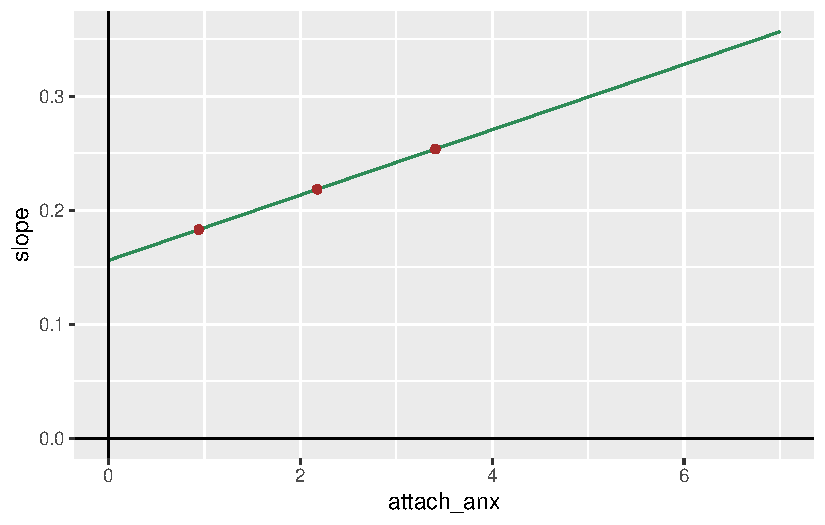
\includegraphics[keepaspectratio]{index_files/figure-pdf/chunk8-1.pdf}}

从上图可以看出，cope\_emo1的简单斜率(绿色直线)从左到右呈增大趋势。若调节变量attach\_anx向左继续减小，cope\_emo1的简单斜率会接近0、乃至等于0、小于0，若调节变量attach\_anx向右继续增大，cope\_emo1的简单斜率会继续增大，且大于0。

尽管我们计算出了简单斜率，但是，我们并不清楚这些简单斜率是否显著(即，是否显著不等于0)，这使得我们无法就简单斜率的变化趋势(例如：简单斜率的方向是否发生了反转)得出准确的结论。\textbf{若调节效应显著，我们需要进行简单斜率分析，简单斜率分析的目的就是检验简单斜率的显著性。}若调节效应不显著，则表明自变量X的效应不会随着W的变化而变化，我们没必要进行简单斜率分析。

\section{简单斜率分析}\label{ux7b80ux5355ux659cux7387ux5206ux6790}

简单斜率分析有两种方法：

选点法(pick-a-point
method)，选点法又被称为聚光灯技术。调节变量的取值可能有无数个，选点法就是选择调节变量的几个有代表性的数值点，然后检验相应的简单斜率的显著性，继而粗略地推断简单斜率的变化趋势。选点法一般选择调节变量的三个点：M-SD，M，M+SD。例如，选择前文slope-attach\_anx图中的三个红色的点进行简单斜率分析。

J-N技术(Johnson-Neyman
technique)，J-N技术又被称为探照灯技术。调节变量的取值可能有无数个，J-N技术就是对调节变量的所有数值进行检验，继而准确地找到调节变量令简单斜率显著的区间范围。例如，对前文slope-attach\_anx图中的绿色直线上的所有点进行简单斜率分析。

实际上，如果选点法选的点足够多，选点法就是J-N技术。所以，简单斜率分析的关键只有一个：当W取特定值时，X的简单斜率的显著性如何检验？下文介绍三种方法：

\begin{enumerate}
\def\labelenumi{\arabic{enumi}.}
\tightlist
\item
  平移坐标法。
\item
  使用emmeans中的emtrends函数。
\item
  在lavaan中定义简单斜率。
\end{enumerate}

\subsection{平移坐标法}\label{ux5e73ux79fbux5750ux6807ux6cd5}

观察前文slope-attach\_anx图，在该图中，slope-attach\_anx直线与y轴的交点(即attach\_anx
=
0时的简单斜率slope的显著性)在回归分析中已经得到了检验。如果我们将slope-attach\_anx坐标系中的y轴向右移动，使我们选择的红色的点(attach\_anx处于低、中、高水平时的简单斜率)落在y轴上，回归分析即可对其简单斜率进行检验。接下来，我们attach\_anx取中等水平(attach\_anx的均值)值时的简单斜率为例进行演示。

\begin{enumerate}
\def\labelenumi{\arabic{enumi}.}
\tightlist
\item
  平移坐标。按照中学时学到的``左加右减''的原理，想令y轴向右移动，那么应使attach\_anx减去移动的距离------attach\_anx的均值。
\end{enumerate}

\begin{Shaded}
\begin{Highlighting}[numbers=left,,]
\NormalTok{depress}\SpecialCharTok{$}\NormalTok{attach\_anx\_translated }\OtherTok{\textless{}{-}}\NormalTok{ depress}\SpecialCharTok{$}\NormalTok{attach\_anx }\SpecialCharTok{{-}} \FunctionTok{mean}\NormalTok{(depress}\SpecialCharTok{$}\NormalTok{attach\_anx, }\AttributeTok{na.rm =} \ConstantTok{TRUE}\NormalTok{)}
\end{Highlighting}
\end{Shaded}

\begin{enumerate}
\def\labelenumi{\arabic{enumi}.}
\setcounter{enumi}{1}
\tightlist
\item
  建立交互项，检验调节效应
\end{enumerate}

\begin{Shaded}
\begin{Highlighting}[numbers=left,,]
\NormalTok{fit\_translated }\OtherTok{\textless{}{-}} \FunctionTok{lm}\NormalTok{(depr1 }\SpecialCharTok{\textasciitilde{}}\NormalTok{ cope\_emo1}\SpecialCharTok{*}\NormalTok{attach\_anx\_translated, depress)}
\FunctionTok{summary}\NormalTok{(fit\_translated)}
\DocumentationTok{\#\# }
\DocumentationTok{\#\# Call:}
\DocumentationTok{\#\# lm(formula = depr1 \textasciitilde{} cope\_emo1 * attach\_anx\_translated, data = depress)}
\DocumentationTok{\#\# }
\DocumentationTok{\#\# Residuals:}
\DocumentationTok{\#\#      Min       1Q   Median       3Q      Max }
\DocumentationTok{\#\# {-}0.75114 {-}0.24216 {-}0.02308  0.25177  0.97300 }
\DocumentationTok{\#\# }
\DocumentationTok{\#\# Coefficients:}
\DocumentationTok{\#\#                                 Estimate Std. Error t value Pr(\textgreater{}|t|)    }
\DocumentationTok{\#\# (Intercept)                      1.35244    0.10546  12.825  \textless{} 2e{-}16 ***}
\DocumentationTok{\#\# cope\_emo1                        0.21837    0.03948   5.531 1.18e{-}07 ***}
\DocumentationTok{\#\# attach\_anx\_translated           {-}0.06087    0.08355  {-}0.728    0.467    }
\DocumentationTok{\#\# cope\_emo1:attach\_anx\_translated  0.02866    0.02946   0.973    0.332    }
\DocumentationTok{\#\# {-}{-}{-}}
\DocumentationTok{\#\# Signif. codes:  0 \textquotesingle{}***\textquotesingle{} 0.001 \textquotesingle{}**\textquotesingle{} 0.01 \textquotesingle{}*\textquotesingle{} 0.05 \textquotesingle{}.\textquotesingle{} 0.1 \textquotesingle{} \textquotesingle{} 1}
\DocumentationTok{\#\# }
\DocumentationTok{\#\# Residual standard error: 0.346 on 170 degrees of freedom}
\DocumentationTok{\#\#   (11 observations deleted due to missingness)}
\DocumentationTok{\#\# Multiple R{-}squared:  0.1754, Adjusted R{-}squared:  0.1609 }
\DocumentationTok{\#\# F{-}statistic: 12.06 on 3 and 170 DF,  p{-}value: 3.399e{-}07}
\end{Highlighting}
\end{Shaded}

上述结果显示，cope\_emo1一次项的回归系数为0.21837, p \textless{}
0.001。0.21837为attach\_anx\_translated =
0时cope\_emo1的简单斜率，当attach\_anx\_translated = 0时，attach\_anx =
attach\_anx\_medium，因此，0.21837为attach\_anx =
attach\_anx\_medium时cope\_emo1的简单斜率。使用同样的方法，我们检验调节变量W取任意值时自变量X的简单斜率。

\subsection{emtrends}\label{emtrends}

我们可以使用emmeans中的emtrends函数进行简单斜率分析：

\begin{Shaded}
\begin{Highlighting}[numbers=left,,]
\NormalTok{simple\_slope\_tests }\OtherTok{\textless{}{-}} \FunctionTok{emtrends}\NormalTok{(}
  \CommentTok{\# 回归分析的结果}
\NormalTok{  fit,}
  \CommentTok{\# 调节变量}
  \AttributeTok{specs =} \StringTok{"attach\_anx"}\NormalTok{,}
  \CommentTok{\# 自变量}
  \AttributeTok{var =} \StringTok{"cope\_emo1"}\NormalTok{,}
  \CommentTok{\# 指定调节变量的取值}
  \AttributeTok{at =} \FunctionTok{list}\NormalTok{(}\AttributeTok{attach\_anx =} \FunctionTok{c}\NormalTok{(}\DecValTok{0}\NormalTok{, attach\_anx\_low, attach\_anx\_medium, attach\_anx\_high)))}
\CommentTok{\# 输出简单斜率检验的结果}
\NormalTok{simple\_slope\_tests}
\DocumentationTok{\#\#  attach\_anx cope\_emo1.trend     SE  df lower.CL upper.CL}
\DocumentationTok{\#\#       0.000           0.156 0.0789 170 0.000388    0.312}
\DocumentationTok{\#\#       0.941           0.183 0.0565 170 0.071473    0.295}
\DocumentationTok{\#\#       2.174           0.218 0.0395 170 0.140437    0.296}
\DocumentationTok{\#\#       3.407           0.254 0.0506 170 0.153760    0.354}
\DocumentationTok{\#\# }
\DocumentationTok{\#\# Confidence level used: 0.95}
\CommentTok{\# 输出简单斜率检验的p值}
\FunctionTok{summary}\NormalTok{(simple\_slope\_tests, }\AttributeTok{infer =} \ConstantTok{TRUE}\NormalTok{)}
\DocumentationTok{\#\#  attach\_anx cope\_emo1.trend     SE  df lower.CL upper.CL t.ratio p.value}
\DocumentationTok{\#\#       0.000           0.156 0.0789 170 0.000388    0.312   1.979  0.0494}
\DocumentationTok{\#\#       0.941           0.183 0.0565 170 0.071473    0.295   3.239  0.0014}
\DocumentationTok{\#\#       2.174           0.218 0.0395 170 0.140437    0.296   5.531 \textless{}0.0001}
\DocumentationTok{\#\#       3.407           0.254 0.0506 170 0.153760    0.354   5.011 \textless{}0.0001}
\DocumentationTok{\#\# }
\DocumentationTok{\#\# Confidence level used: 0.95}
\end{Highlighting}
\end{Shaded}

\subsection{基于lavaan}\label{ux57faux4e8elavaan}

前文我们基于\texttt{lm()}进行调节效应检验与简单斜率分析，但\texttt{lm()}只能处理一个回归方程，当涉及包含多个回归方程的复杂模型时，我们可以使用\texttt{lavaan}进行调节效应检验与简单斜率分析。下面我们演示\texttt{lavaan}的做法：

\begin{Shaded}
\begin{Highlighting}[numbers=left,,]
\CommentTok{\# 界定模型}
\NormalTok{model }\OtherTok{\textless{}{-}} \StringTok{"}
\StringTok{depr1 \textasciitilde{} b1*cope\_emo1 + b2*attach\_anx + b3*cope\_emo1:attach\_anx}
\StringTok{\# 定义简单斜率}
\StringTok{\# 调节变量attach\_anx的特定取值由前文计算得到}
\StringTok{slope\_l := b1 + b3*0.9598129}
\StringTok{slope\_m := b1 + b3*2.173759}
\StringTok{slope\_h := b1 + b3*3.387705}
\StringTok{"}
\NormalTok{fit\_lavaan }\OtherTok{\textless{}{-}} \FunctionTok{sem}\NormalTok{(model, depress)}
\FunctionTok{summary}\NormalTok{(fit\_lavaan)}
\DocumentationTok{\#\# lavaan 0.6{-}21 ended normally after 1 iteration}
\DocumentationTok{\#\# }
\DocumentationTok{\#\#   Estimator                                         ML}
\DocumentationTok{\#\#   Optimization method                           NLMINB}
\DocumentationTok{\#\#   Number of model parameters                         4}
\DocumentationTok{\#\# }
\DocumentationTok{\#\#                                                   Used       Total}
\DocumentationTok{\#\#   Number of observations                           174         185}
\DocumentationTok{\#\# }
\DocumentationTok{\#\# Model Test User Model:}
\DocumentationTok{\#\#                                                       }
\DocumentationTok{\#\#   Test statistic                                 0.000}
\DocumentationTok{\#\#   Degrees of freedom                                 0}
\DocumentationTok{\#\# }
\DocumentationTok{\#\# Parameter Estimates:}
\DocumentationTok{\#\# }
\DocumentationTok{\#\#   Standard errors                             Standard}
\DocumentationTok{\#\#   Information                                 Expected}
\DocumentationTok{\#\#   Information saturated (h1) model          Structured}
\DocumentationTok{\#\# }
\DocumentationTok{\#\# Regressions:}
\DocumentationTok{\#\#                    Estimate  Std.Err  z{-}value  P(\textgreater{}|z|)}
\DocumentationTok{\#\#   depr1 \textasciitilde{}                                             }
\DocumentationTok{\#\#     cope\_emo1 (b1)    0.156    0.078    2.002    0.045}
\DocumentationTok{\#\#     attach\_nx (b2)   {-}0.061    0.083   {-}0.737    0.461}
\DocumentationTok{\#\#     cp\_m1:tt\_ (b3)    0.029    0.029    0.984    0.325}
\DocumentationTok{\#\# }
\DocumentationTok{\#\# Variances:}
\DocumentationTok{\#\#                    Estimate  Std.Err  z{-}value  P(\textgreater{}|z|)}
\DocumentationTok{\#\#    .depr1             0.117    0.013    9.327    0.000}
\DocumentationTok{\#\# }
\DocumentationTok{\#\# Defined Parameters:}
\DocumentationTok{\#\#                    Estimate  Std.Err  z{-}value  P(\textgreater{}|z|)}
\DocumentationTok{\#\#     slope\_l           0.184    0.055    3.309    0.001}
\DocumentationTok{\#\#     slope\_m           0.218    0.039    5.595    0.000}
\DocumentationTok{\#\#     slope\_h           0.253    0.050    5.095    0.000}
\end{Highlighting}
\end{Shaded}

上述结果与前文基于\texttt{lm()}的结果在统计结论上是一致的，统计结果数值上的细微差异可忽略不计。

\section{调节效应图}\label{ux8c03ux8282ux6548ux5e94ux56fe}

为了更清楚的描述依恋焦虑对情绪应对与抑郁的关系的调节作用，我们有必要作调节效应图。调节效应图分别作出当调节变量W取低、中、高水平值时X预测Y的直线。一种比较直接的做法是我们直接将X(自变量，横坐标)与W(调节变量)的特定取值代入回归方程，然后计算出Y(结果变量，纵坐标)的值，之后我们基于XWY的数据用ggplot2或者其他作图软件(例如：WPS)作图。另一种方式是使用\texttt{emmean}程序包中的\texttt{emmip()}函数作调节效应图。\texttt{emmip()}函数作调节效应图的代码如下，其中的参数\texttt{formula}的界定方法有些特殊：\texttt{\textasciitilde{}}左侧是调节变量，而不是结果变量。

\begin{Shaded}
\begin{Highlighting}[numbers=left,,]
\FunctionTok{emmip}\NormalTok{(}
\NormalTok{  fit,}
  \CommentTok{\# 注意下面的表达式：trace.factors(调节变量) \textasciitilde{} x.factors(自变量)}
  \AttributeTok{formula =}\NormalTok{ attach\_anx }\SpecialCharTok{\textasciitilde{}}\NormalTok{ cope\_emo1,}
  \CommentTok{\# 指定调节变量的取值}
  \AttributeTok{at =} \FunctionTok{list}\NormalTok{(}
    \AttributeTok{cope\_emo1 =} \FunctionTok{c}\NormalTok{(}\DecValTok{1}\NormalTok{, }\DecValTok{7}\NormalTok{),}
    \AttributeTok{attach\_anx =} \FunctionTok{c}\NormalTok{(attach\_anx\_low, attach\_anx\_medium, attach\_anx\_high))}
\NormalTok{)}
\end{Highlighting}
\end{Shaded}

\pandocbounded{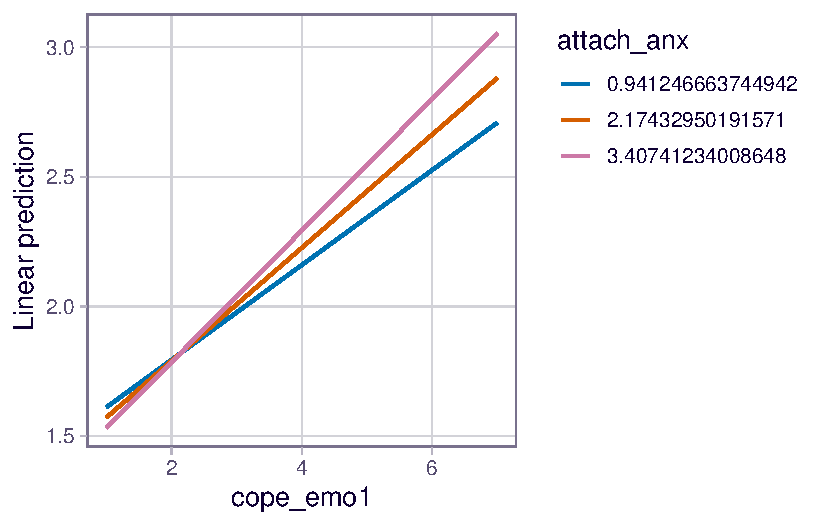
\includegraphics[keepaspectratio]{index_files/figure-pdf/chunk13-1.pdf}}

\section{中心化}\label{ux4e2dux5fc3ux5316}

过去的文献要求在建立交互项之前，需要先进行中心化，理由是``中心化可以避免多重共线性''，这一观点已经被证明是错误的。但是，中心化确实还是有好处的，它的好处在于``使截距有意义''。下面我们先对数据进行中心化，然后再进行调节效应检验、简单斜率分析，并作图。

\begin{Shaded}
\begin{Highlighting}[numbers=left,,]
\CommentTok{\# 使用Keng程序包中的Scale函数对自变量与调节变量进行中心化}
\NormalTok{depress}\SpecialCharTok{$}\NormalTok{cope\_emo1\_c }\OtherTok{\textless{}{-}}\NormalTok{ Keng}\SpecialCharTok{::}\FunctionTok{Scale}\NormalTok{(depress}\SpecialCharTok{$}\NormalTok{cope\_emo1, }\AttributeTok{m =} \DecValTok{0}\NormalTok{)}
\NormalTok{depress}\SpecialCharTok{$}\NormalTok{attach\_anx\_c }\OtherTok{\textless{}{-}}\NormalTok{ Keng}\SpecialCharTok{::}\FunctionTok{Scale}\NormalTok{(depress}\SpecialCharTok{$}\NormalTok{attach\_anx, }\AttributeTok{m =} \DecValTok{0}\NormalTok{)}
\CommentTok{\# 检验调节效应}
\NormalTok{fit2 }\OtherTok{\textless{}{-}} \FunctionTok{lm}\NormalTok{(depr1 }\SpecialCharTok{\textasciitilde{}}\NormalTok{ cope\_emo1\_c}\SpecialCharTok{*}\NormalTok{attach\_anx\_c, depress)}
\FunctionTok{summary}\NormalTok{(fit2)}
\DocumentationTok{\#\# }
\DocumentationTok{\#\# Call:}
\DocumentationTok{\#\# lm(formula = depr1 \textasciitilde{} cope\_emo1\_c * attach\_anx\_c, data = depress)}
\DocumentationTok{\#\# }
\DocumentationTok{\#\# Residuals:}
\DocumentationTok{\#\#      Min       1Q   Median       3Q      Max }
\DocumentationTok{\#\# {-}0.75114 {-}0.24216 {-}0.02308  0.25177  0.97300 }
\DocumentationTok{\#\# }
\DocumentationTok{\#\# Coefficients:}
\DocumentationTok{\#\#                          Estimate Std. Error t value Pr(\textgreater{}|t|)    }
\DocumentationTok{\#\# (Intercept)               1.91941    0.02652  72.372  \textless{} 2e{-}16 ***}
\DocumentationTok{\#\# cope\_emo1\_c               0.21837    0.03948   5.531 1.18e{-}07 ***}
\DocumentationTok{\#\# attach\_anx\_c              0.01355    0.02202   0.615    0.539    }
\DocumentationTok{\#\# cope\_emo1\_c:attach\_anx\_c  0.02866    0.02946   0.973    0.332    }
\DocumentationTok{\#\# {-}{-}{-}}
\DocumentationTok{\#\# Signif. codes:  0 \textquotesingle{}***\textquotesingle{} 0.001 \textquotesingle{}**\textquotesingle{} 0.01 \textquotesingle{}*\textquotesingle{} 0.05 \textquotesingle{}.\textquotesingle{} 0.1 \textquotesingle{} \textquotesingle{} 1}
\DocumentationTok{\#\# }
\DocumentationTok{\#\# Residual standard error: 0.346 on 170 degrees of freedom}
\DocumentationTok{\#\#   (11 observations deleted due to missingness)}
\DocumentationTok{\#\# Multiple R{-}squared:  0.1754, Adjusted R{-}squared:  0.1609 }
\DocumentationTok{\#\# F{-}statistic: 12.06 on 3 and 170 DF,  p{-}value: 3.399e{-}07}
\CommentTok{\# 调节变量attach\_anx\_c的低、中、高水平值}
\NormalTok{attach\_anx\_cl }\OtherTok{\textless{}{-}} \SpecialCharTok{{-}}\FunctionTok{sd}\NormalTok{(depress}\SpecialCharTok{$}\NormalTok{attach\_anx\_c, }\AttributeTok{na.rm =} \ConstantTok{TRUE}\NormalTok{)}
\NormalTok{attach\_anx\_cm }\OtherTok{\textless{}{-}} \DecValTok{0}
\NormalTok{attach\_anx\_ch }\OtherTok{\textless{}{-}} \FunctionTok{sd}\NormalTok{(depress}\SpecialCharTok{$}\NormalTok{attach\_anx\_c, }\AttributeTok{na.rm =} \ConstantTok{TRUE}\NormalTok{)}
\CommentTok{\# 简单斜率检验}
\NormalTok{simple\_slope\_tests2 }\OtherTok{\textless{}{-}} \FunctionTok{emtrends}\NormalTok{(}
  \CommentTok{\# 回归分析的结果}
\NormalTok{  fit2,}
  \CommentTok{\# 调节变量}
  \AttributeTok{specs =} \StringTok{"attach\_anx\_c"}\NormalTok{,}
  \CommentTok{\# 自变量}
  \AttributeTok{var =} \StringTok{"cope\_emo1\_c"}\NormalTok{,}
  \CommentTok{\# 指定调节变量的取值}
  \AttributeTok{at =} \FunctionTok{list}\NormalTok{(}\AttributeTok{attach\_anx\_c =} \FunctionTok{c}\NormalTok{(attach\_anx\_cl, attach\_anx\_cm, attach\_anx\_ch)))}
\CommentTok{\# 输出简单斜率检验的结果}
\FunctionTok{summary}\NormalTok{(simple\_slope\_tests2, }\AttributeTok{infer =} \ConstantTok{TRUE}\NormalTok{)}
\DocumentationTok{\#\#  attach\_anx\_c cope\_emo1\_c.trend     SE  df lower.CL upper.CL t.ratio p.value}
\DocumentationTok{\#\#         {-}1.23             0.183 0.0565 170   0.0715    0.295   3.239  0.0014}
\DocumentationTok{\#\#          0.00             0.218 0.0395 170   0.1404    0.296   5.531 \textless{}0.0001}
\DocumentationTok{\#\#          1.23             0.254 0.0506 170   0.1538    0.354   5.011 \textless{}0.0001}
\DocumentationTok{\#\# }
\DocumentationTok{\#\# Confidence level used: 0.95}
\CommentTok{\# 作调节效应图}
\FunctionTok{emmip}\NormalTok{(}
\NormalTok{  fit2,}
  \CommentTok{\# 注意下面的表达式：trace.factors(调节变量) \textasciitilde{} x.factors(自变量)}
  \AttributeTok{formula =}\NormalTok{ attach\_anx\_c }\SpecialCharTok{\textasciitilde{}}\NormalTok{ cope\_emo1\_c,}
  \CommentTok{\# 指定调节变量的取值}
  \AttributeTok{at =} \FunctionTok{list}\NormalTok{(}
    \AttributeTok{cope\_emo1\_c =} \FunctionTok{c}\NormalTok{(}\DecValTok{1}\NormalTok{, }\DecValTok{7}\NormalTok{),}
    \AttributeTok{attach\_anx\_c =} \FunctionTok{c}\NormalTok{(attach\_anx\_cl, attach\_anx\_cm, attach\_anx\_ch))}
\NormalTok{)}
\end{Highlighting}
\end{Shaded}

\pandocbounded{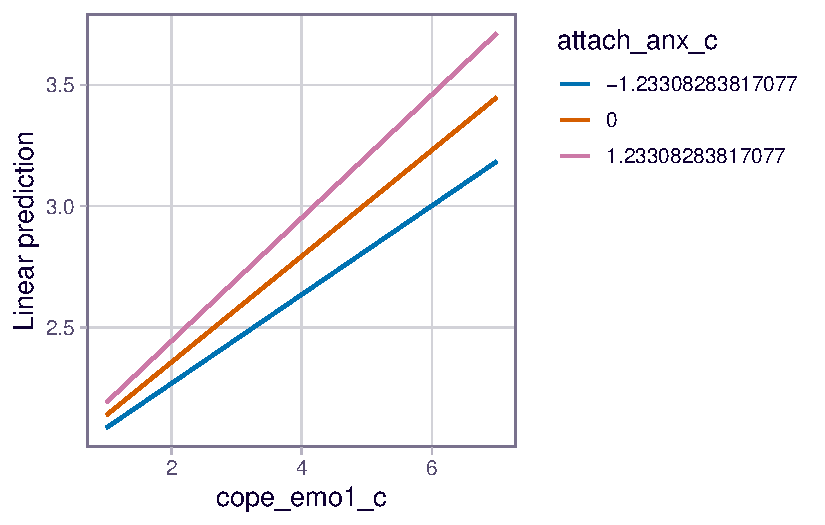
\includegraphics[keepaspectratio]{index_files/figure-pdf/chunk14-1.pdf}}

\section{标准化}\label{ux6807ux51c6ux5316}

与中介效应不同，由于涉及到交互项，调节模型的标准化回归系数的计算要稍微复杂些。标准化回归分析就是先将变量进行标准化，然后再进行回归分析。这一定义对于调节模型依然适用。只是需要注意，我们应当先将变量进行标准化，然后再计算交互项；而不能先计算交互项，然后再将变量标准化。在统计软件的眼中，交互项与自变量、调节变量一样，只是一列数据而已，因此，统计软件进行标准化回归分析时会按部就班的先把交互项标准化、再进行回归分析，因此，统计软件自动输出的标准化回归是错的，我们不能直接使用。接下来，我们对调节模型进行标准化的回归分析，从而得到标准化的回归系数：

\begin{Shaded}
\begin{Highlighting}[numbers=left,,]
\CommentTok{\# 使用Keng中的Scale函数对变量进行标准化}
\NormalTok{depress}\SpecialCharTok{$}\NormalTok{cope\_emo1\_z }\OtherTok{\textless{}{-}}\NormalTok{ Keng}\SpecialCharTok{::}\FunctionTok{Scale}\NormalTok{(depress}\SpecialCharTok{$}\NormalTok{cope\_emo1, }\AttributeTok{m =} \DecValTok{0}\NormalTok{, }\AttributeTok{sd =} \DecValTok{1}\NormalTok{)}
\NormalTok{depress}\SpecialCharTok{$}\NormalTok{attach\_anx\_z }\OtherTok{\textless{}{-}}\NormalTok{ Keng}\SpecialCharTok{::}\FunctionTok{Scale}\NormalTok{(depress}\SpecialCharTok{$}\NormalTok{attach\_anx, }\AttributeTok{m =} \DecValTok{0}\NormalTok{, }\AttributeTok{sd =} \DecValTok{1}\NormalTok{)}
\NormalTok{depress}\SpecialCharTok{$}\NormalTok{depr1\_z }\OtherTok{\textless{}{-}}\NormalTok{ Keng}\SpecialCharTok{::}\FunctionTok{Scale}\NormalTok{(depress}\SpecialCharTok{$}\NormalTok{depr1, }\AttributeTok{m =} \DecValTok{0}\NormalTok{, }\AttributeTok{sd =} \DecValTok{1}\NormalTok{)}
\CommentTok{\# 调节效应检验}
\NormalTok{fit3 }\OtherTok{\textless{}{-}} \FunctionTok{lm}\NormalTok{(depr1\_z }\SpecialCharTok{\textasciitilde{}}\NormalTok{ cope\_emo1\_z}\SpecialCharTok{*}\NormalTok{attach\_anx\_z, depress)}
\CommentTok{\# 输出结果}
\FunctionTok{summary}\NormalTok{(fit3)}
\DocumentationTok{\#\# }
\DocumentationTok{\#\# Call:}
\DocumentationTok{\#\# lm(formula = depr1\_z \textasciitilde{} cope\_emo1\_z * attach\_anx\_z, data = depress)}
\DocumentationTok{\#\# }
\DocumentationTok{\#\# Residuals:}
\DocumentationTok{\#\#      Min       1Q   Median       3Q      Max }
\DocumentationTok{\#\# {-}1.98865 {-}0.64111 {-}0.06111  0.66657  2.57603 }
\DocumentationTok{\#\# }
\DocumentationTok{\#\# Coefficients:}
\DocumentationTok{\#\#                          Estimate Std. Error t value Pr(\textgreater{}|t|)    }
\DocumentationTok{\#\# (Intercept)              {-}0.01010    0.07022  {-}0.144    0.886    }
\DocumentationTok{\#\# cope\_emo1\_z               0.39263    0.07098   5.531 1.18e{-}07 ***}
\DocumentationTok{\#\# attach\_anx\_z              0.04422    0.07188   0.615    0.539    }
\DocumentationTok{\#\# cope\_emo1\_z:attach\_anx\_z  0.06354    0.06533   0.973    0.332    }
\DocumentationTok{\#\# {-}{-}{-}}
\DocumentationTok{\#\# Signif. codes:  0 \textquotesingle{}***\textquotesingle{} 0.001 \textquotesingle{}**\textquotesingle{} 0.01 \textquotesingle{}*\textquotesingle{} 0.05 \textquotesingle{}.\textquotesingle{} 0.1 \textquotesingle{} \textquotesingle{} 1}
\DocumentationTok{\#\# }
\DocumentationTok{\#\# Residual standard error: 0.916 on 170 degrees of freedom}
\DocumentationTok{\#\#   (11 observations deleted due to missingness)}
\DocumentationTok{\#\# Multiple R{-}squared:  0.1754, Adjusted R{-}squared:  0.1609 }
\DocumentationTok{\#\# F{-}statistic: 12.06 on 3 and 170 DF,  p{-}value: 3.399e{-}07}
\end{Highlighting}
\end{Shaded}

\section{三元调节效应}\label{ux4e09ux5143ux8c03ux8282ux6548ux5e94}

包含三元调节效应的回归方程如下：

\[
Y = b0 + b1*X + b2*W + b3*V + b4*X*W + b5*X*V + b6*W*V + b7*X*W*V
\]

在上式中，
b1*X是X的一次项，b4*X*W是X与W的二次项，b7*X*W*V是X、W、V的三次项。我们对X合并同类项，得到:

\[
Y = (b0 + b2*W + b3*V + b6*W*V) + (b1 + b4*W + b5*V + b7*W*V)*X
\]

可得，

\begin{enumerate}
\def\labelenumi{\arabic{enumi}.}
\tightlist
\item
  X对Y的效应为(b1 + b4*W + b5*V + b7*W*V)。
\item
  X对Y的效应是关于变量W与V的函数，会随着W与V的变化而变化。
\item
  三元调节效应成立的根据是回归系数b7，若b7显著，则三元调节效应显著，若b7不显著，则三元调节效应不存在。
\end{enumerate}

既然b7是检验三元调节效应的关键，我们是否可以将其他的一次项、二次项从回归方程中剔除呢？不可以，当保留三次项时，二次项与一次项应当同时保留。若三元调节效应不存在，我们可以将X、W、V的三次项从回归模型中剔除，只保留一次项与二次项，然后检验二元调节效应是否显著。若二元调节效应不存在，我们可以将相应的二次项从回归模型中剔除，仅检验一次项的显著性。

三元调节效应的检验方法与简单斜率分析的方法与二元调节效应基本一致，读者自行摸索，本文不再赘述。

\section{涉及分类变量的调节效应}\label{ux6d89ux53caux5206ux7c7bux53d8ux91cfux7684ux8c03ux8282ux6548ux5e94}

\subsection{调节变量是二分变量}\label{ux8c03ux8282ux53d8ux91cfux662fux4e8cux5206ux53d8ux91cf}

若调节变量是二分变量，例如，性别，此时调节效应检验与简单斜率分析的方法与连续变量没有区别，只是需要注意，简单斜率分析在选点时要选择有意义的点。例如gender的取值为1与2，那么，选点法只需要选两个点，gender
= 1，gender = 2。其他的点没有意义。

\subsection{调节变量是多分类变量}\label{ux8c03ux8282ux53d8ux91cfux662fux591aux5206ux7c7bux53d8ux91cf}

与回归分析一致，此时，我们需要对多分类变量进行虚拟编码。例如，以depress数据为例，class有4个水平，我们需要将其编码为3个虚拟变量class3，class5，class9。调节效应如何检验呢？当调节变量只有一个W时，我们需要建立自变量X与W的交互项XW；此时，我们的调节变量class用3个虚拟变量class3、class5、class9表示，要检验class的调节效应，我们需要建立X与三个虚拟变量的交互项，并将它们同时纳入回归方程中。其他统计分析的步骤无需多言。

全文到此结束。




\end{document}
